% -----------------------------------------------------------------
% Document class: Article
\documentclass[ a4paper, twoside, 11pt]{article}
\usepackage{../../../macros-general}
\usepackage{../../../macros-article}
% Number of the handout, quiz, exam, etc.
\newcommand{\numero}{04}
\setcounter{numero}{\numero}

% -----------------------------------------------------------------
\begin{document}
\allowdisplaybreaks

\begin{center}
\Large Mec\'anica Vectorial (MECG-1001): Trabajo Aut\'onomo \numero \\[2ex]
\small \textbf{Semestre:} 2017-2018 T\'ermino II \qquad
\textbf{Instructor:} Luis I. Reyes Castro \qquad
\textbf{Paralelo:} 09
\end{center}
\fullskip

% =============================================
\begin{problem}
\textbf{[4 Puntos]} Los carros de carreras $A$ y $B$ se desplazan sobre porciones circulares de una pista. En el instante que se indica, la rapidez de $A$ disminuye a raz\'on de 7 m/s\tsup{2} y la rapidez de $B$ se incrementa a una tasa de 2 m/s\tsup{2}. Para las posiciones mostradas, determine \textit{(i)} la velocidad de
$B$ relativa a $A$, y \textit{(ii)} la aceleraci\'on de $B$ relativa a $A$.

\begin{figure}[htb]
\centering
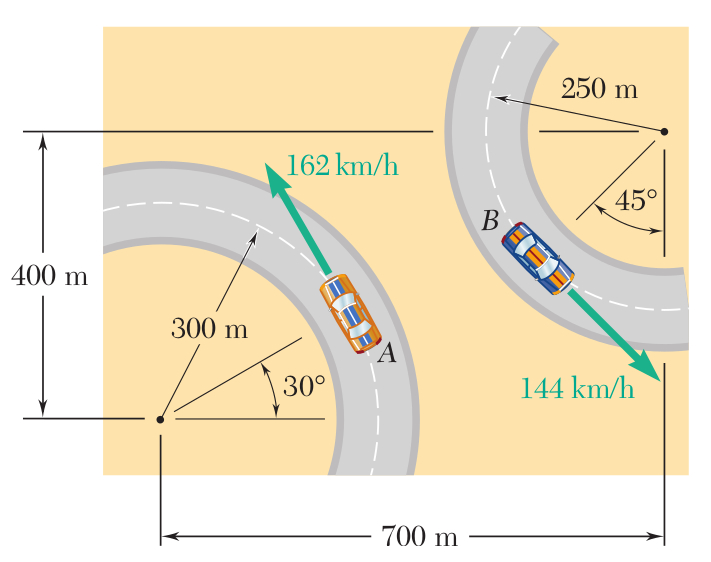
\includegraphics[width=0.5\textwidth]{problema-1.jpg}
\end{figure}

\emph{Soluci\'on:} Primero, los vectores unitarios para el caso del carro $A$ son: 
\begin{align*}
\vec{e_t} \; & = \; ( \, -\cos(60\deg), \, +\sin(60\deg) \, )
\; = \; ( \, -0.500, \, +0.866) \\
\vec{e_n} \; & = \; ( \, -\cos(30\deg), \, -\sin(30\deg) \, )
\; = \; ( \, -0.866, \, -0.500)
\end{align*}
Dado que $v_A = 45$ m/s tenemos: 
\[
\vec{v_A} \; = \; 45 \, \vec{e_t}
\; = \; ( \, -22.50, \, +38.97) \; \text{m/s}
\]
Adem\'as, puesto que $\dot{v}_A = -7$ m/s\tsup{2} y que $\rho_A = 300$ m, tenemos: 
\begin{align*}
\vec{a_A} \; & = \;
\dot{v}_A \, \vec{e_t} + \frac{v_A^2}{\rho_A} \, \vec{e_n} \\
& = \; -7 \, ( \, -0.500, \, +0.866)
+ \frac{45^2}{300} \, ( \, -0.866, \, -0.500) \\[1ex]
& = \; ( \, -2.3455, \, -9.437 \, ) \; \text{m/s\tsup{2}}
\end{align*}

Segundo, los vectores unitarios para el caso del carro $B$ son: 
\begin{align*}
\vec{e_t} \; & = \; ( \, -\cos(45\deg), \, -\sin(45\deg) \, )
\; = \; ( \, +0.707, \, -0.707) \\
\vec{e_n} \; & = \; ( \, +\cos(45\deg), \, +\sin(45\deg) \, )
\; = \; ( \, +0.707, \, +0.707)
\end{align*}
Dado que $v_B = 40$ m/s tenemos: 
\[
\vec{v_B} \; = \; 40 \, \vec{e_t}
\; = \; ( \, +28.28, \, -28.28) \; \text{m/s}
\]
Adem\'as, puesto que $\dot{v}_B = +2$ m/s\tsup{2} y que $\rho_B = 250$ m, tenemos: 
\begin{align*}
\vec{a_B} \; & = \;
\dot{v}_B \, \vec{e_t} + \frac{v_B^2}{\rho_B} \, \vec{e_n} \\
& = \; +2 \, ( \, +0.707, \, -0.707)
+ \frac{40^2}{250} \, ( \, +0.707, \, +0.707) \\[1ex]
& = \; ( \, +5.9388, \, +3.1108 \, ) \; \text{m/s\tsup{2}}
\end{align*}

Finalmente: 
\begin{align*}
\vec{v_{B/A}} \; & = \; \vec{v_B} - \vec{v_A}
\; = \; ( \, +50.78, \, -67.25 \, ) \; \text{m/s}
\; \equiv \; 84.27 \; \text{m/s} \; \measuredangle \; -52.94\deg \\
\vec{a_{B/A}} \; & = \; \vec{a_B} - \vec{a_A}
\; = \; ( \, +8.2843, \, +12.548 \, ) \; \text{m/s\tsup{2}}
\; \equiv \; 15.036 \; \text{m/s\tsup{2}} \; \measuredangle \; +56.57\deg
\end{align*}

\end{problem}
\fullskip

% =============================================
\begin{problem}
\textbf{[4 Puntos]} La varilla $AB$ se mueve sobre una peque\~na rueda en $C$ mientras el extremo $A$ se desplaza hacia la derecha con una velocidad constante de 500 mm/s. En el instante mostrado, determine \textit{(i)} la velocidad angular de la varilla y \textit{(ii)} la velocidad del extremo $B$ de la varilla.

\begin{figure}[htb]
\centering
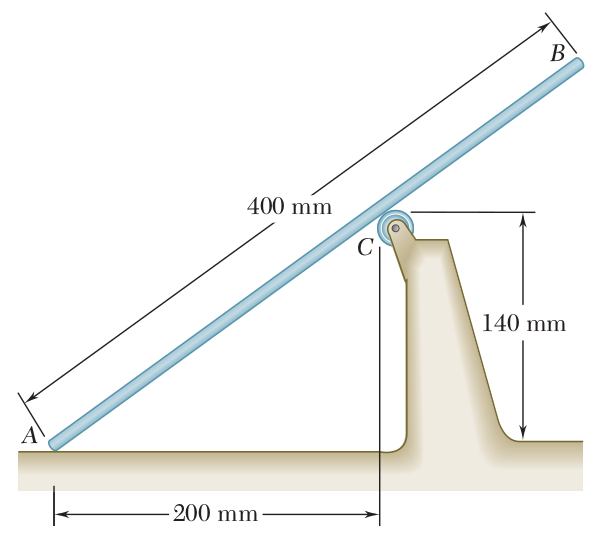
\includegraphics[width=0.5\textwidth]{problema-2.jpg}
\end{figure}

\emph{Soluci\'on:} Primero reconocemos que: 
\[
\vec{v_A} \; = \; ( \, +0.500, 0 \, ) \; \text{m/s}
\]
Luego observamos que el \'angulo de la varilla con la horizontal es: 
\[
\theta \; = \; \tan^{-1}(140/200) \; = \; 34.99\deg \approx 35 \deg
\]
Consecuentemente: 
\begin{align*}
\vec{\hat{r}_{AB}} \; & = \;
( \, +\cos(\theta), \, +\sin(\theta) \, ) \; = \;
( \, +0.819, \, +0.573 \, ) \\
\vec{r_{AB}} \; & = \; 0.400 \, \vec{\hat{r}_{AB}} \; = \;
( \, +0.3277, \, +0.2294 \, ) \; \text{m} \\
\vec{r_{AC}} \; & = \; ( \, 0.200, \, 0.140 \, ) \; \text{m}
\end{align*}

Ahora utilizamos la condici\'on de rodadura en $C$ para reconocer que la velocidad en $C$ es paralela a la varilla. \Iec
\[
\vec{v_C}
\; = \; v_C \, \vec{\hat{r}_{AB}}
\; = \; ( \, +0.819 \, v_C, \, +0.573 \, v_C \, )
\]
Entonces, de la relaci\'on entre las velocidades de $A$ y $C$ obtenemos: 
\begin{align*}
& \vec{v_C} \; = \; \vec{v_A} + \vec{\omega} \times \vec{r_{AC}} \\[1ex]
& \Longrightarrow \; \left[ \begin{array}{c}
+0.819 \, v_C \\ +0.573 \, v_C
\end{array} \right] \; = \;
\left[ \begin{array}{c}
+0.500 \\ 0
\end{array} \right] + 
\left[ \begin{array}{c}
-0.140 \, \omega \\ +0.200 \, \omega
\end{array} \right] \\[1ex]
& \Longrightarrow \; v_C \; = \; 0.349 \, \omega \\
& \Longrightarrow \; \vec{\omega} \; = \; +1.1741 \, \vec{\hat{k}} \; \text{rad/s}
\end{align*}
Finalmente, calculamos la velocidad en $B$ considerando la velocidad en $A$ :
\begin{align*}
& \vec{v_B} \; = \; \vec{v_A} + \vec{\omega} \times \vec{r_{AB}} \\[1ex]
& \Longrightarrow \; \left[ \begin{array}{c}
+(v_B)_x \\ +(v_B)_y
\end{array} \right] \; = \;
\left[ \begin{array}{c}
+0.500 \\ 0
\end{array} \right] + 
\left[ \begin{array}{c}
(-0.2294)(1.1741) \\ (+0.3277)(1.1741)
\end{array} \right] \\[1ex]
& \Longrightarrow \; \vec{v_B} \; = \; 
\left[ \begin{array}{c}
+0.2307 \\ +0.3848
\end{array} \right] \, \text{m/s}
\end{align*}

\end{problem}
\fullskip

\end{document}